\documentclass[a4paper,openany]{uantwerpenassignment}

\usepackage[dutch]{babel}
\usepackage{titlesec}
\usepackage{tikz}
\usepackage{pythonhighlight}
\usepackage{amsmath}
\usepackage{array}

\newenvironment{conditions}
  {\par\vspace{\abovedisplayskip}\noindent\begin{tabular}{>{$}l<{$} @{${}={}$} l}}
  {\end{tabular}\par\vspace{\belowdisplayskip}}

\definecolor{code}{HTML}{ecf0f1}
\definecolor{codetext}{HTML}{d9534f}
\newcommand{\codeword}[1]{
    \colorbox{code}{\texttt{\textcolor{codetext}{#1}}}
}

\newcommand{\reference}[1]{\textit{\ref{#1}. \nameref{#1}}}

\definecolor{code}{HTML}{ecf0f1}
\definecolor{codetext}{HTML}{d9534f}
\newcommand{\codeword}[1]{
    \colorbox{code}{\texttt{\textcolor{codetext}{#1}}}
}

\facultyacronym{TI}

\title{\sffamily Chess AI-Agent}
\subtitle{\sffamily5-Artificiële Intelligentie}
\author{\sffamily Mathias Maes, Tijs Van Alphen \\en Willem Van der Elst}

\programme{BA}{IW}{EI}

\academicyear{2020-2021}

\publisher{}

\titleformat{\chapter}{\sffamily\huge\bfseries}{\thechapter.}{10pt}{\sffamily\huge\bfseries}
\titleformat{\section}{\sffamily\LARGE\bfseries}{\thesection.}{10pt}{\sffamily\LARGE\bfseries}
\titleformat{\subsection}{\sffamily\Large\bfseries}{\thesubsection.}{10pt}{\sffamily\Large\bfseries}
\titleformat{\subsubsection}{}{}{10pt}{\sffamily\large\bfseries}


\begin{document}

\sffamily
\maketitle

\tableofcontents

\chapter{Keuze}

Het type AI was een belangrijke keuze van dit project. Het moest haalbaar zijn om te implementeren binnen de beperkte tijdsperiode en we moesten onze eigen niet-supercomputers gebruiken om te treinen. Een lijst  met de voor- en nadelen van de verschillende opties werd opgesteld.\\[2 \baselineskip]


\textbf{Search}:\\
Er zijn te veel mogelijke states ($\approx10^{120}$) om de hele tree uit te werken. 

\textbf{Multi-Agent search} (Minimax, Alpha-Beta pruning):\\
Deze methode wordt gebruikt door meerdere bronnen, maar we hebben er nog geen ervaring mee. 

\textbf{Reinforcement learning} (Generalised Q learning):\\
We hebben dit al gebruikt en daarom begrijpen we het al en kunnen we het snel implementeren.\\
Eenmaal getraind, zal het optimaal functioneren. De training heeft echter veel tijd nodig en de keuze van de features is niet zo voor de hand liggend.

\textbf{Neural network/ Deep learning:}
Onze ervaring met Deep learning is nogal beperkt. We weten niet goed wat we als in- en output moeten nemen. \\[2 \baselineskip]


Q-Learning leek ons het interessantst, maar Minimax is haalbaarder en zou sowieso een goed resultaat leveren. Uiteindelijk besloten we om beide methodes uit te werken. We hadden namelijk een thesis\cite{rl} gevonden die een minimax agent gebruikte als feature voor een generalized Q-Learner.

\chapter{Alpha-Beta Pruning}

\section{Utility}
\label{utility}

Onze utility maakt gebruik van veel kenmerken van de features van onze Q-Learner dus gaan we dit later behandelen.
Je kan op het moment onze utility als volgt begrijpen:

$$
u(S) = 
\begin{cases}
    100 &\mbox{Als je gewonnen hebt}\\
    -30 &\mbox{Als er een stalemate gespeeld is}\\
    -100 &\mbox{Als je verloren hebt}\\
    c + C + \Delta M + \Delta m + s + f_q &\mbox{Bij overige situaties}
\end{cases}
$$

\begin{conditions}
    c & Of er gecastled is met de vorige move\\
    C & Of het bord in schaak staat\\
    \Delta M & Het materiaal verschil op het bord\\
    \Delta m & Het verschil in mobility\\
    s & De positie score voor alle eigen stukken\\
    f_q & Een gewogen(geleerd of niet-geleerd) aantal features
\end{conditions}

Hoe deze kleine sub-functies bepaald worden wordt later nog besproken in het stuk \reference{features}.

\chapter{Q-Learning Agent}

\section{Generalization}

De eerste agent die we moesten maken was de Q-agent deze is generalized omdat zoals bij de minpunten stonden van general search algoritmes, is het bijna onmogelijk om elke staat te bezoeken. Daarom dat we niet gewoon Q-learning gaan doen maar generalized Q-learning.

\section{Features}
\label{features}

We hebben een hoop features gedefinieerd deze zijn voornamelijk gebaseerd op de paper\cite{rl} die we gevonden hebben. De bedoeling van deze features is om een state zo goed mogelijk te definiëren. Je kan hieronder een beschrijving vinden van elks van onze 55 features.

We berekenen onze features als volt:

$$
Q(s,a) = \sum_{i} w_{i} \cdot \sigma \left( f_i(s, a)\right)
$$

De $\sigma(x)$ die we in de berekening zien wordt als volgt gedefinieerd:

$$
\sigma(x) = \frac{2}{1 + e^{-x}} - 1
$$

Dit is een aangepaste versie van de bekende sigmoid\cite{WSF} functie. Onze versie zorgt in tegenstelling tot de originele er voor dat waardes in het interval $\left]-1,1\right[$ vallen.\\
Hier zie je de grafiek van de functie:

\begin{figure}[h]
    \centering
    \begin{tikzpicture}[scale=2]
        \draw[->] (-2, 0) -- (2, 0) node[right] {$x$};
        \draw[->] (0, -1.2) -- (0, 1.2) node[above] {$y$};

        \draw[dashed] (-2, 0.5) -- (2, 0.5);
        \node (A) at (-2, 0.6) {\tiny $1$};

        \draw[dashed] (-2, -0.5) -- (2, -0.5);
        \node (B) at (-2, -0.6) {\tiny $-1$};

        \draw[scale=0.5, domain=-3.9:3.9, smooth, variable=\x, blue] plot ({\x}, { 2/(1 + exp(-\x)) - 1 });
        \node[blue] (C) at (0.4, 0.32) {$\sigma$};
    \end{tikzpicture}
    \caption{$\sigma(x)$} \label{fig:sigmoid}
\end{figure}



\subsection{Material}
We definiëren elke soort schaakstuk met een waarde, op deze manier kunnen we de stukken onderscheiden t.o.v. elkaar. Zo krijgt de koningin een hogere waarde dan een pion, omdat deze meer van waarde is voor ons dan een pion. Hier zie je hoe de schaakstukken zich verhouden t.o.v. elkaar.

\begin{python}
def getMaterialValue(piece_type):
    if piece_type is chess.PAWN:
        return 1
    elif piece_type is chess.KNIGHT or piece_type is chess.BISHOP:
        return 3
    elif piece_type is chess.ROOK:
        return 5
    elif piece_type is chess.QUEEN:
        return 9
    elif piece_type is chess.KING:
        return 10

    return 0
\end{python}

\subsection{Amount of Pieces}
Een andere feature die we gebruiken is het aantal soort stukken van elke speler. We doen dit 1 keer voor alle schaakstukken van het bord, zowel de onze als die van de tegenspeler. 

We creëerden ook voor elke type schaakstuk 2 features. Eén die bijhoud hoeveel van dit type schaakstukken je zelf op het bord bevindt en één die bijhield hoeveel je opponent er heeft. Op deze manier zal onze Q-agent leren dat een slecht ding is als de opponent veel stukken van een type en dat het goed is als je zelf veel schaakstukken bezit.

Het laatste wat we ook nakijken is de feature \codeword{AmountBalancePieces()} deze zal de material value van alle stukken van de speler berekenen en de material value van de tegenspeler er af trekken. Wanneer dit getal dus negatief is betekend dat dat de tegenspeler globaal bekeken er beter voor staat als jezelf.

\subsection{Mobility}
De \codeword{Mobility.py} file berekent voor elke type schaakstuk hoeveel vakjes het stuk kan bereiken. 

Dit wordt gebruikt voor de mobility features. Hierbij gaan we voor elke type schaakstuk kijken op hoeveel vakjes die kan terechtkomen. Dit zullen we ook weer doen voor zowel de speler als de tegenspeler.

De feature \codeword{MobilityRookS()} zal voor elke Rook (toren) van de eigen speler (S in de functie staat voor self) berekenen op hoeveel vakjes die kan komen en bij elkaar optellen.

Voor het berekenen van de vakjes gaan kijken of een een legal move zou zijn als we dat stuk naar een vakje zouden zetten, wanneer dit een false teruggeeft betekend het dat we niet naar dat vakje kunnen omdat er al een ander van je schaakstukken op staat. Hier hebben we wat problemen ondervonden voor de opponent omdat we enkel onze eigen stukken kunnen verplaatsen. Onze oplossing hiervoor was een copy van het bord maken gevolgd door een board turn, op deze manier speel je dan zogezegd even als de opponent op het gekopieerde bord. 

\subsection{Attackers}
\subsection{Forks}
\subsection{Control}
\subsubsection{Center Control}
\subsubsection{Board Control}

\section{Reward}


Evaluation\cite{chessprogramming}

\chapter{Optimalisaties}

We hebben een hoop optimalisaties moeten toevoegen aan onze Q-Learner om hem zo rap mogelijk te laten denken.

\section{Multi-Threading}

We hebben multi-threading toegevoegd aan onze q-learner zo berekent hij de q-waarde van elke actie in een aparte thread. We hebben bewust niet gekozen om elke feature apart omdat dit onze timing issues verergerde in plaat van verbeterde.

We hebben door multi-threading onze iteratie tijd met 20\% weten dalen.

Hier zie je de resultaten van het processor gebruik:

\begin{figure}[h]
    \centering
    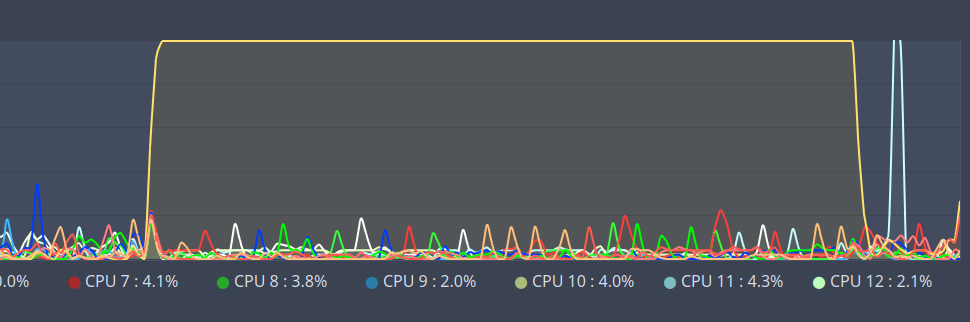
\includegraphics[width=300pt]{images/singlethreaded.png}
    \caption{Single Threaded Q-Learner CPU usage}
    \label{fig:singlethreaded}
\end{figure}

\begin{figure}[h]
    \centering
    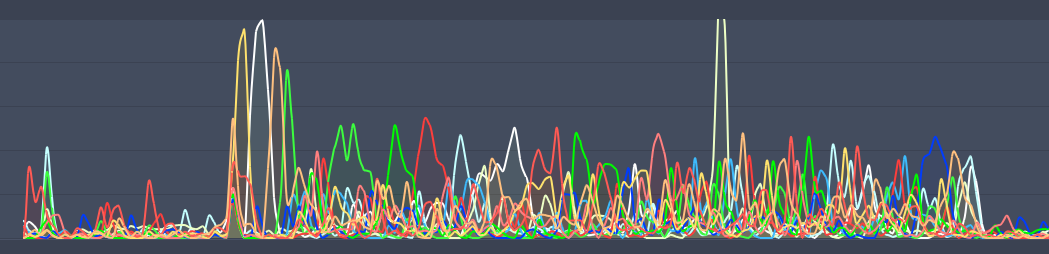
\includegraphics[width=350pt]{images/multithreaded.png}
    \caption{Multi Threaded Q-Learner CPU usage}
    \label{fig:multithreaded}
\end{figure}

\section{Caching}

We gebruiken ook veel plaatsen caching zodat we niet 2 keer hetzelfde moeten uitrekenen. De meest bijzondere cache is deze voor onze alpha-beta feature, deze moet per bord state maar 1 keer uitvoeren waardoor we de alpha-beta langer kunnen laten zoeken en een hoop tijd besparen.
Det tijd die we hierdoor besparen per iteratie kan soms tot een minuut of 2 oplopen.

\chapter{Resultaten}
\section{GrandQ vs. Stockfish (0-544)}

Command:\\
\codeword{python3 train -o stockfish --skill 0 --depth 10 -tt 5 -dt 0 -e 0.3 -d 0.6 -l 0.01 -q -i -1}

\section{GrandQ vs. Alpha-Beta (544 - 5732)}

Command:\\
\codeword{python3 train -o ab --depth 10 -tt 5 -dt 0 -e 0.3 -d 0.6 -l 0.01 -q -i -1}

Command na ongveer 1500 episodes:\\
\codeword{python3 train -o ab --depth 10 -tt 5 -dt 0 -e 0.2 -d 0.4 -l 0.01 -q -i -1}

\bibliography{sources}
\bibliographystyle{ieeetr}

\end{document}
